\usetikzlibrary{shadings,shadows,shapes.arrows}

\begin{tikzpicture}
	\def\k{1.2}
	\node (e) at (0,0*\k) {$e$};
 	\node (d1) at (-1,-1*\k) {$d_1$};
 	\node (d2) at (1,-1*\k) {$d_2$};
	\node (c) at (0,-2*\k) {$c$};
 	\node (b1) at (-1,-3*\k) {$b_1$};
 	\node (b2) at (1,-3*\k) {$b_2$};
 	\node (a) at (0,-4*\k){$a$};
 	
 	\path[->] (e) edge node {} (d1);
 	\path[->] (e) edge node {} (d2);
 	\path[<-] (c) edge node {} (d1);
 	\path[<-] (c) edge node {} (d2);
 	\path[->] (c) edge node {} (b1);
 	\path[->] (c) edge node {} (b2);
 	\path[<-] (a) edge node {} (b1);
 	\path[<-] (a) edge node {} (b2);
 	
 	\def\p{5}
	\node (e) at (0+\p,0*\k) {$8$};
 	\node (d1) at (-1+\p,-1*\k) {$-1$};
 	\node (d2) at (1+\p,-1*\k) {$2$};
	\node (c) at (0+\p,-2*\k) {$4$};
 	\node (b1) at (-1+\p,-3*\k) {$5$};
 	\node (b2) at (1+\p,-3*\k) {$7$};
 	\node (a) at (0+\p,-4*\k){$3$};
 	
 	\tikzstyle{le}=[left,blue,xshift=-10,font=\small]
 	\tikzstyle{re}=[right,blue,xshift=14,font=\small]
 	\path[->] (e) edge node [le] {$ \cfrac{\partial e}{\partial d_1}(-1,2)$} (d1);
 	\path[->] (e) edge node [re] {$\cfrac{\partial e}{\partial d_2}(-1,2)$} (d2);
 	\path[<-] (c) edge node [le] {$\cfrac{de}{dc}(4)$} (d1);
 	\path[<-] (c) edge node [re] {$\cfrac{de}{dc}(4)$} (d2);
 	\path[->] (c) edge node [le] {$\cfrac{\partial e}{\partial b_1}(5,7)$} (b1);
 	\path[->] (c) edge node [re] {$\cfrac{\partial e}{\partial b_2}(5,7)$} (b2);
 	\path[<-] (a) edge node [le] {$\cfrac{de}{da}(3)$} (b1);
 	\path[<-] (a) edge node [re] {$\cfrac{de}{da}(3)$} (b2);
 	
	\node[single arrow,
		    single arrow head extend=1em,
		    inner sep=0.5em,
		    draw=black,
		    fill=black!10,
		    minimum height=15em,
		    left color=white,
		    right color=cyan,
		    drop shadow,
		    shape border rotate=270] at (8.3,-2*\k) {};
\end{tikzpicture}
